\documentclass{standalone}
\usepackage{tikz}
\usetikzlibrary{patterns, positioning}
\usepackage[sfdefault]{ClearSans} %% option 'sfdefault' activates Clear Sans as the default text font
\usepackage[T1]{fontenc}

\begin{document}
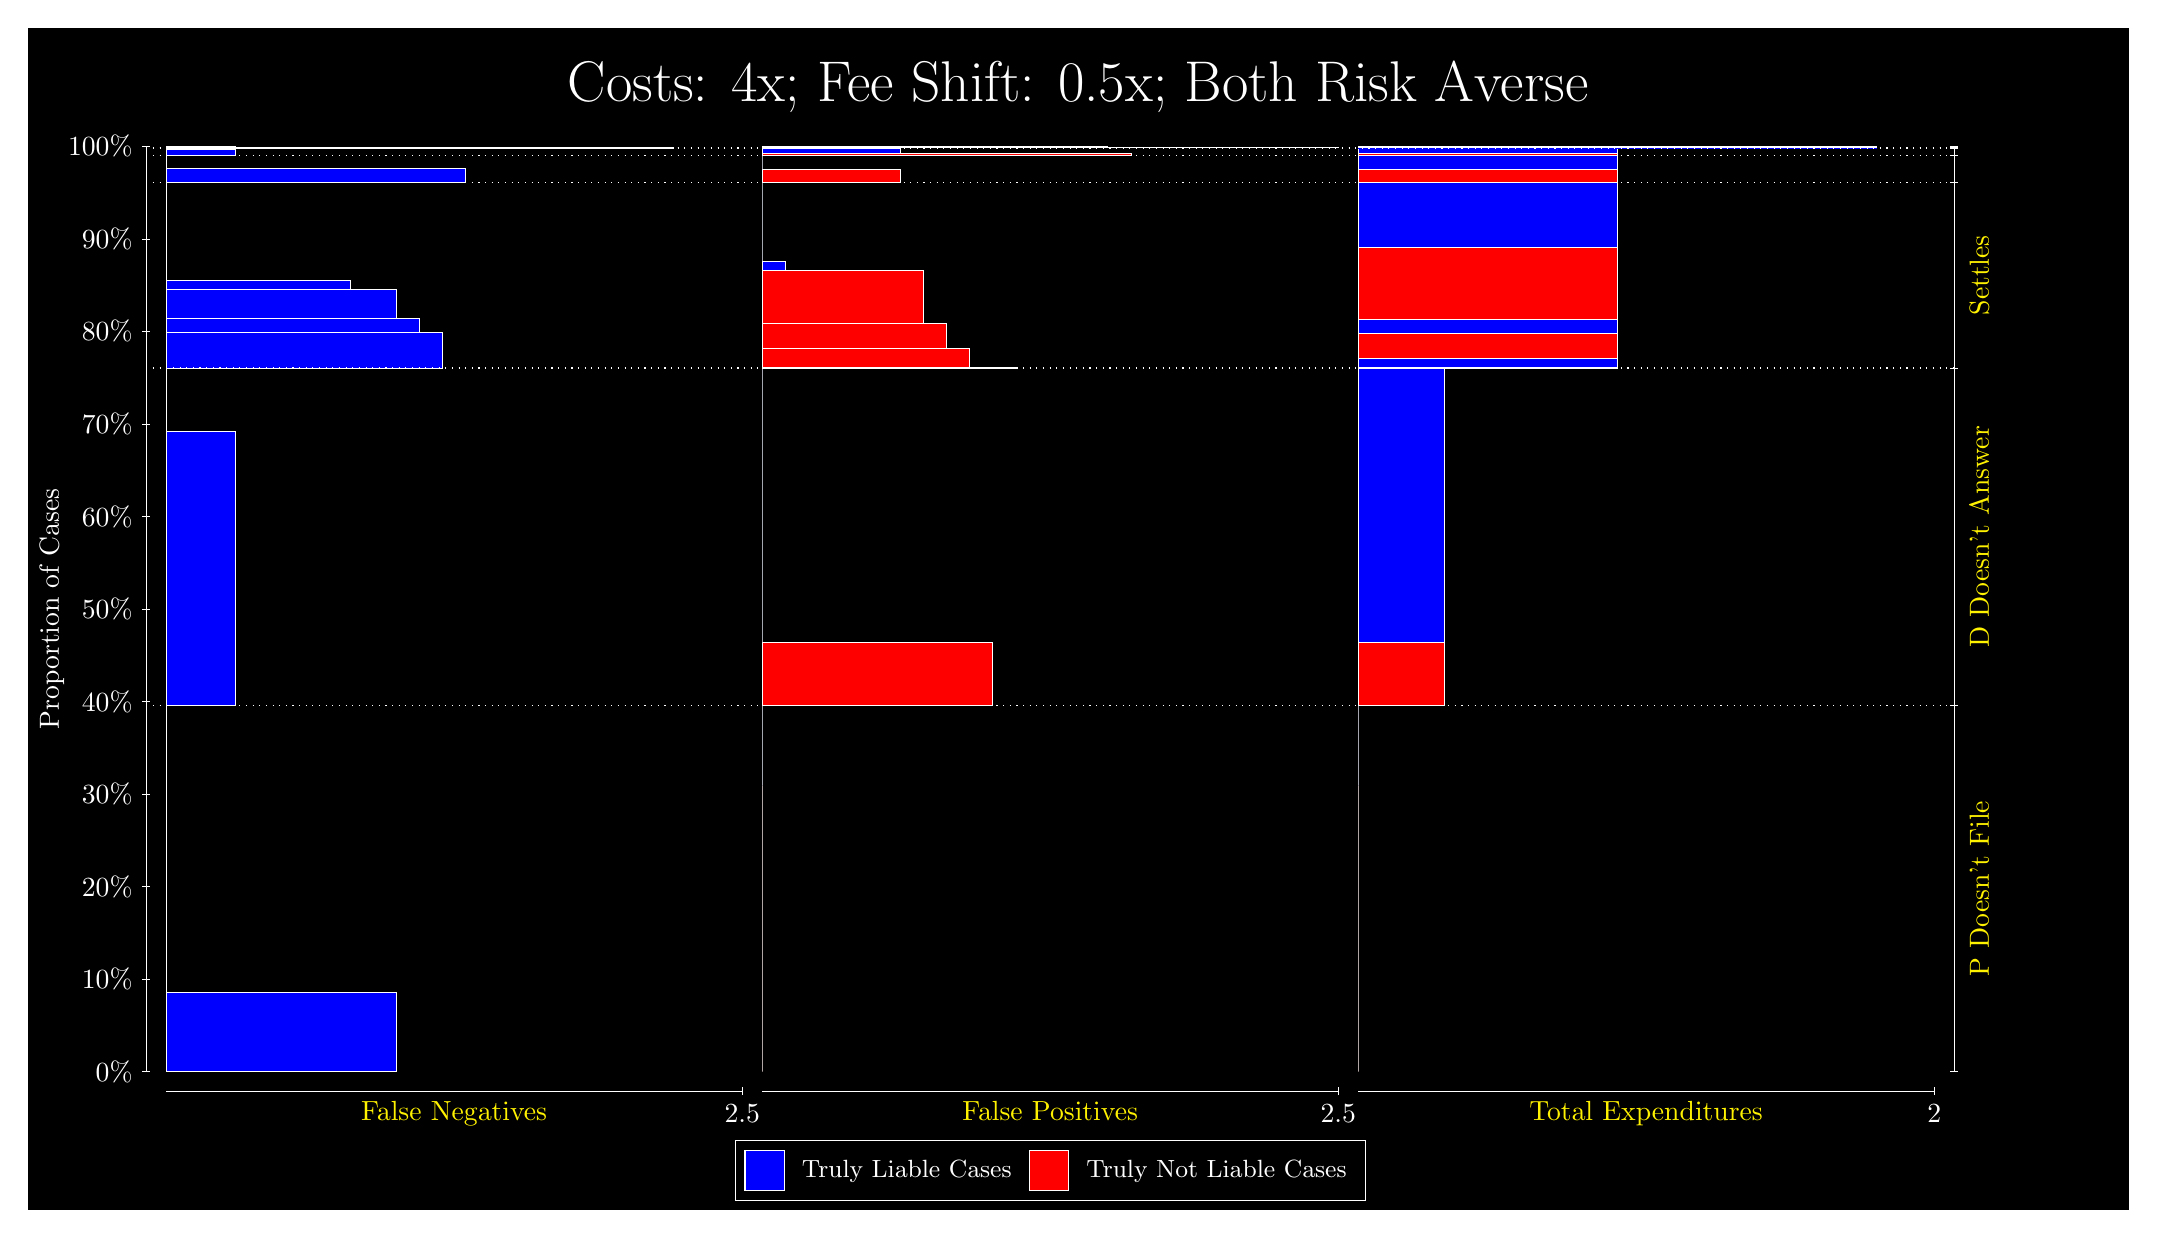
\begin{tikzpicture}
\draw[fill=black] (0,0) rectangle (26.667,15);
\draw[text=white] (0,13.5) rectangle (26.667,15) node[midway] {\huge Costs: 4x; Fee Shift: 0.5x; Both Risk Averse};
\draw[white, very thin] (1.5,1.75) -- (1.5,13.5);
\node[rotate=90, text=white, anchor=center] at (0.3, 7.625) {Proportion of Cases};
\draw[white, very thin] (1.45,1.75) -- (1.55,1.75);
\node[text=white, anchor=east] at (1.45, 1.75) {0\%};
\draw[white, very thin] (1.45,2.925) -- (1.55,2.925);
\node[text=white, anchor=east] at (1.45, 2.925) {10\%};
\draw[white, very thin] (1.45,4.1) -- (1.55,4.1);
\node[text=white, anchor=east] at (1.45, 4.1) {20\%};
\draw[white, very thin] (1.45,5.275) -- (1.55,5.275);
\node[text=white, anchor=east] at (1.45, 5.275) {30\%};
\draw[white, very thin] (1.45,6.45) -- (1.55,6.45);
\node[text=white, anchor=east] at (1.45, 6.45) {40\%};
\draw[white, very thin] (1.45,7.625) -- (1.55,7.625);
\node[text=white, anchor=east] at (1.45, 7.625) {50\%};
\draw[white, very thin] (1.45,8.8) -- (1.55,8.8);
\node[text=white, anchor=east] at (1.45, 8.8) {60\%};
\draw[white, very thin] (1.45,9.975) -- (1.55,9.975);
\node[text=white, anchor=east] at (1.45, 9.975) {70\%};
\draw[white, very thin] (1.45,11.15) -- (1.55,11.15);
\node[text=white, anchor=east] at (1.45, 11.15) {80\%};
\draw[white, very thin] (1.45,12.325) -- (1.55,12.325);
\node[text=white, anchor=east] at (1.45, 12.325) {90\%};
\draw[white, very thin] (1.45,13.5) -- (1.55,13.5);
\node[text=white, anchor=east] at (1.45, 13.5) {100\%};

\draw[white, very thin] (24.457,1.75) -- (24.457,13.5);
\draw[white, very thin] (24.407,1.75) -- (24.507,1.75);
\node[anchor=west] at (24.407, 1.75) {};
\draw[white, very thin] (24.407,6.3955) -- (24.507,6.3955);
\node[anchor=west] at (24.407, 6.3955) {};
\draw[white, very thin] (24.407,10.685) -- (24.507,10.685);
\node[anchor=west] at (24.407, 10.685) {};
\draw[white, very thin] (24.407,13.042) -- (24.507,13.042);
\node[anchor=west] at (24.407, 13.042) {};
\draw[white, very thin] (24.407,13.389) -- (24.507,13.389);
\node[anchor=west] at (24.407, 13.389) {};
\draw[white, very thin] (24.407,13.479) -- (24.507,13.479);
\node[anchor=west] at (24.407, 13.479) {};
\draw[white, very thin] (24.407,13.485) -- (24.507,13.485);
\node[anchor=west] at (24.407, 13.485) {};
\draw[white, very thin] (24.407,13.5) -- (24.507,13.5);
\node[anchor=west] at (24.407, 13.5) {};

\draw[white, very thin, fill=blue] (1.75,1.75) rectangle (4.6775,2.7616);
\draw[white, very thin, fill=red] (1.75,2.7616) rectangle (1.75,6.3955);
\draw[white, very thin, fill=blue] (1.75,6.3955) rectangle (2.6283,9.8803);
\draw[white, very thin, fill=red] (1.75,9.8803) rectangle (1.75,10.685);
\draw[white, very thin, fill=blue] (1.75,10.685) rectangle (5.2631,11.142);
\draw[white, very thin, fill=blue] (1.75,11.142) rectangle (4.9703,11.317);
\draw[white, very thin, fill=blue] (1.75,11.317) rectangle (4.6775,11.685);
\draw[white, very thin, fill=blue] (1.75,11.685) rectangle (4.3848,11.689);
\draw[white, very thin, fill=blue] (1.75,11.689) rectangle (4.092,11.796);
\draw[white, very thin, fill=red] (1.75,11.796) rectangle (1.75,13.042);
\draw[white, very thin, fill=blue] (1.75,13.042) rectangle (5.5558,13.226);
\draw[white, very thin, fill=red] (1.75,13.226) rectangle (1.75,13.389);
\draw[white, very thin, fill=blue] (1.75,13.389) rectangle (2.6283,13.459);
\draw[white, very thin, fill=red] (1.75,13.459) rectangle (1.75,13.479);
\draw[white, very thin, fill=blue] (1.75,13.479) rectangle (8.1906,13.482);
\draw[white, very thin, fill=red] (1.75,13.482) rectangle (1.75,13.485);
\draw[white, very thin, fill=blue] (1.75,13.485) rectangle (2.6283,13.497);
\draw[white, very thin, fill=red] (1.75,13.497) rectangle (1.75,13.5);
\draw[white, very thin, fill=red] (9.3189,1.75) rectangle (9.3189,5.3838);
\draw[white, very thin, fill=blue] (9.3189,5.3838) rectangle (9.3189,6.3955);
\draw[white, very thin, fill=red] (9.3189,6.3955) rectangle (12.246,7.2006);
\draw[white, very thin, fill=blue] (9.3189,7.2006) rectangle (9.3189,10.685);
\draw[white, very thin, fill=red] (9.3189,10.685) rectangle (12.539,10.698);
\draw[white, very thin, fill=red] (9.3189,10.698) rectangle (12.246,10.7);
\draw[white, very thin, fill=red] (9.3189,10.7) rectangle (11.954,10.935);
\draw[white, very thin, fill=red] (9.3189,10.935) rectangle (11.661,11.257);
\draw[white, very thin, fill=red] (9.3189,11.257) rectangle (11.368,11.932);
\draw[white, very thin, fill=blue] (9.3189,11.932) rectangle (9.6116,12.039);
\draw[white, very thin, fill=blue] (9.3189,12.039) rectangle (9.3189,13.042);
\draw[white, very thin, fill=red] (9.3189,13.042) rectangle (11.075,13.205);
\draw[white, very thin, fill=blue] (9.3189,13.205) rectangle (9.3189,13.389);
\draw[white, very thin, fill=red] (9.3189,13.389) rectangle (14.003,13.409);
\draw[white, very thin, fill=blue] (9.3189,13.409) rectangle (11.075,13.479);
\draw[white, very thin, fill=red] (9.3189,13.479) rectangle (11.075,13.482);
\draw[white, very thin, fill=blue] (9.3189,13.482) rectangle (9.3189,13.485);
\draw[white, very thin, fill=red] (9.3189,13.485) rectangle (16.638,13.488);
\draw[white, very thin, fill=blue] (9.3189,13.488) rectangle (13.71,13.5);
\draw[white, very thin, fill=red] (16.888,1.75) rectangle (16.888,5.3838);
\draw[white, very thin, fill=blue] (16.888,5.3838) rectangle (16.888,6.3955);
\draw[white, very thin, fill=red] (16.888,6.3955) rectangle (17.986,7.2006);
\draw[white, very thin, fill=blue] (16.888,7.2006) rectangle (17.986,10.685);
\draw[white, very thin, fill=red] (16.888,10.685) rectangle (20.181,10.698);
\draw[white, very thin, fill=blue] (16.888,10.698) rectangle (20.181,10.805);
\draw[white, very thin, fill=red] (16.888,10.805) rectangle (20.181,11.127);
\draw[white, very thin, fill=blue] (16.888,11.127) rectangle (20.181,11.302);
\draw[white, very thin, fill=red] (16.888,11.302) rectangle (20.181,12.214);
\draw[white, very thin, fill=blue] (16.888,12.214) rectangle (20.181,13.042);
\draw[white, very thin, fill=red] (16.888,13.042) rectangle (20.181,13.205);
\draw[white, very thin, fill=blue] (16.888,13.205) rectangle (20.181,13.389);
\draw[white, very thin, fill=red] (16.888,13.389) rectangle (20.181,13.409);
\draw[white, very thin, fill=blue] (16.888,13.409) rectangle (20.181,13.479);
\draw[white, very thin, fill=red] (16.888,13.479) rectangle (23.475,13.482);
\draw[white, very thin, fill=blue] (16.888,13.482) rectangle (23.475,13.485);
\draw[white, very thin, fill=red] (16.888,13.485) rectangle (23.475,13.488);
\draw[white, very thin, fill=blue] (16.888,13.488) rectangle (23.475,13.5);
\draw[white, dotted] (1.5,6.3955) -- (24.457,6.3955);
\draw[white, dotted] (1.5,10.685) -- (24.457,10.685);
\draw[white, dotted] (1.5,13.042) -- (24.457,13.042);
\draw[white, dotted] (1.5,13.389) -- (24.457,13.389);
\draw[white, dotted] (1.5,13.479) -- (24.457,13.479);
\draw[white, dotted] (1.5,13.485) -- (24.457,13.485);
\draw[white, very thin] (1.75,1.5) -- (9.0689,1.5);
\node[text=yellow, anchor=north] at (5.4094, 1.5) {False Negatives};
\draw[white, very thin] (9.0689,1.45) -- (9.0689,1.55);
\node[text=white, anchor=north] at (9.0689, 1.45) {2.5};

\draw[white, very thin] (9.3189,1.5) -- (16.638,1.5);
\node[text=yellow, anchor=north] at (12.978, 1.5) {False Positives};
\draw[white, very thin] (16.638,1.45) -- (16.638,1.55);
\node[text=white, anchor=north] at (16.638, 1.45) {2.5};

\draw[white, very thin] (16.888,1.5) -- (24.207,1.5);
\node[text=yellow, anchor=north] at (20.547, 1.5) {Total Expenditures};
\draw[white, very thin] (24.207,1.45) -- (24.207,1.55);
\node[text=white, anchor=north] at (24.207, 1.45) {2};

\node[text=yellow, centered, rotate=90] at (24.777, 4.0727) {P Doesn't File};
\node[text=yellow, centered, rotate=90] at (24.777, 8.5405) {D Doesn't Answer};
\node[text=yellow, centered, rotate=90] at (24.777, 11.864) {Settles};





\draw (12.978300999999998,1.5) node[draw=none] (baseCoordinate) {};
\begin{scope}[align=center]
        \matrix[scale=0.5, draw=white, below=0.5cm of baseCoordinate, nodes={draw}, column sep=0.1cm]{
            \node[rectangle, draw, minimum width=0.5cm, minimum height=0.5cm, fill=blue] {}; &
            \node[draw=none, font=\small, text=white] (B) {Truly Liable Cases}; &
            \node[rectangle, draw, minimum width=0.5cm, minimum height=0.5cm, fill=red] {}; &
            \node[draw=none, font=\small, text=white] (B) {Truly Not Liable Cases}; \\
            };
\end{scope}

\end{tikzpicture}
\end{document}